\section{M\'EMOIRE SCIENTIFIQUE}
\label{sec:memoire}

\ANRinfo{Maximum 5 pages. On donne ci-dessous des indications sur le contenu possible du mémoire. Ce mémoire peut être accompagné de rapports annexes plus détaillés.\\}

\ANRinfo{Le mémoire scientifique couvre la totalité de la durée du projet. Il doit présenter une synthèse auto-suffisante rappelant les objectifs, le travail réalisé et les résultats obtenus mis en perspective avec les attentes initiales et l’état de l’art. C’est un document d’un format semblable à celui des articles scientifiques ou des monographies. Il doit refléter le caractère collectif de l’effort fait par les partenaires au cours du projet. Le coordinateur prépare ce rapport sur la base des contributions de tous les partenaires. Une version préliminaire en est soumise à l’ANR pour la revue de fin de projet.\\} 

\ANRinfo{Un mémoire scientifique signalé comme confidentiel ne sera pas diffusé. Justifier brièvement la raison de la confidentialité demandée. Les mémoires non confidentiels seront susceptibles d’être diffusés par l’ANR, notamment via les archives ouvertes http://hal.archives-ouvertes.fr.
}

\subsection*{Mémoire scientifique confidentiel :  non}

\subsection{Résumé du mémoire}

Le projet MAESTRIA avait l'ambition de développer des méthodes automatiques pour l'analyse de la grande quantité d'images satellites hétérogènes d'observation de la Terre disponibles. Il présentait deux objectifs stratégiques principaux :
\paragraph{D'un point de vue méthodologique,} il visait à intégrer les informations extraites de toutes les sources de données disponibles (à la fois les images satellites et les cartes d'occupation du sol existantes), afin d'atténuer les limitations actuelles. En pratique, on visait à améliorer à la fois la précision sémantique et spatiale des cartes d'occupation des sols (OCS) actuelles
(10$\:$m$\rightarrow$ 2-5$\:$m, répondant à la plupart des besoins de suivis environnementaux). En particulier, on comptait aboutir à  une carte OCS générique complète de la France avec une qualité homogène (pour toutes les classes d'intérêt), à différentes périodes de l'année, sans se fonder sur des données de référence récentes. Cela passait par de nouvelles méthodes de fusion d'images multi-sources et multi-échelles. Les énormes quantités de données disponibles devaient être fusionnées de manière parcimonieuse afin d'en tirer les informations pertinentes pour les étapes suivantes de classification pixellaire, en trouvant un compromis entre la précision des résultats de classification et passage à l'échelle des méthodes. Cette étape était vue comme cruciale pour gagner en flexibilité et dériver une plus grande gamme de produits OCS pertinents par la suite.

\paragraph{Dans un esprit applicatif,} MAESTRIA visait à étendre les produits OCS classiques et rigides à une variété plus grande (cartographie de l'utilisation des sols, dérivation de produits à grande échelle, cohérents avec les systèmes continentaux existants) \ldots. Cela soulevait des questions méthodologiques fondamentales afin de répondre aux exigences des différents utilisateurs finaux identifiés à des échelles locale, régionale et nationale. On estimait également important de dériver, à partir de ces couches "centrales", plusieurs sous-produits sur une large gamme de résolutions spatiales (2$\rightarrow$100$\:$m). On souhaitait enfin impliquer des utilisateurs finaux, liés à la surveillance de l'environnement, à l'estimation des ressources naturelles ou à la modélisation du climat, pour obtenir des spécifications particulières de produits OCS à façon.

\subsection{Enjeux et problématique, état de l’art}

\paragraph{Situation en 2018.} Au cours des quinze dernières années, de plus en plus d'initiatives avaient été prises pour la surveillance de l'état et du changement de la couverture terrestre. Il existait en 2018 des bases de données OCS, à différentes échelles spatiales, correspondant à divers besoins des politiques. En général, plus la résolution spatiale est fine, plus l'ensemble des classes est important. Les produits à l'échelle mondiale/continentale ont une précision spatiale limitée (>30$\:$m) mais avec peu de détails thématiques. Ils étaient produits avec des outils de classification automatique à partir d'une ou deux sources de données de télédétection. Un important travail de correction manuelle explique le délai important entre deux dates (>5$\:$ans). Les bases de données nationales sur l'occupation du sol offraient l'avantage d'une meilleure homogénéité et d'une précision spatiale et sémantique améliorées, puisqu'elles sont générées par des organismes faisant autorité. Cependant, elles étaient rarement produites à l'aide d'outils de classification automatique, et la plupart du temps,
avec une seule source de données . Le changement de nomenclature et la mise à jour rapide n'étaient pas possibles et réduisaient drastiquement leur potentiel d'exploitation.

\paragraph{Solutions adoptées alors.} Des cartes mondiales de la couverture terrestre à 20-30$\:$m ont été produites au cours des deux dernières décennies (Europe, Chine, États-Unis), ainsi qu'une nouvelle version de l'European Corine Land Cover, en utilisant des images satellites. Cependant, elles présentaient une très faible précision à la fois en termes de résolution spatiale et de sémantique, et avec toujours un degré élevé d'intervention humaine. De tels produits LC ont été mis à disposition, souvent gratuitement, mais ils sont trop spécifiques (une seule échelle spatiale - grossière -  et un seul ensemble de classes - génériques).\\
L'adaptation des données aux besoins spécifiques (échelle spatiale, ensemble de classes) était un sujet de recherche important, à la fois pour mieux alimenter les modèles environnementaux existants et pour développer de nouveaux services adaptés aux besoins. Des efforts récents en télédétection avaient été consacrés à l'utilisation conjointe des informations spatiales et spectrales et à la gestion du grand nombre de caractéristiques multimodales avec un nombre limité d'échantillons d'apprentissage
d'entraînement. Si la communauté scientifique avait obtenu des résultats  importants, la plupart de ces méthodes ne s'adaptaient pas bien au grand volume de pixels à traiter dans le cadre d'un scénario à l'échelle nationale. En conséquence, les méthodes conventionnelles d'OCS et les avancées récentes dans les méthodes d'apprentissage n'étaient pas adaptées aux nouveaux défis : plus de données, plus d'hétérogénéité, mise à jour fréquente, amélioration spatiale, l'amélioration spatiale, l'extensibilité et l'automatisation.\\
Un premier pas dans cette direction était le développement de la chaîne prototype $\iota^2$ (CESBIO). Cette chaîne est développée
afin de générer des cartes de l'occupation du sol à l'échelle d'un pays à partir d'images de séries temporelles à haute résolution (à savoir les images Sentinel-2). Il était possible d'obtenir des cartes d'une résolution allant jusqu'à 10 mètres avec un ensemble de 15 à 20 classes. $\iota^2$ offrait la possibilité d'intégrer des méthodes de l'état de l'art en classification supervisée et en extraction d'informations à partir d'une base de données topographique existante imparfaite. $\iota^2$ était actuellement mis en œuvre dans le \href{https://www.theia-land.fr/pole-theia-2/}{pôle de données Théia}, mais nécessitait encore d'importants efforts de recherche pour gagner en précision et en flexibilité.

\subsection{Approche scientifique et technique}
\label{subsec:wp}
L'ambition du projet MAESTRIA reposait sur des innovations méthodologiques liées à l'exploitation de grandes quantités de données d'observation de la Terre pour la génération de cartes de l'occupation du sol qui répondent au mieux aux exigences des utilisateurs finaux.
En termes de méthodes, la fusion de données par l'extraction et la représentation de caractéristiques, l'apprentissage et la classification à large échelle sur des données bruitées, ainsi que l'analyse multi-échelles, sont des challenges interdépendants lorsqu'il s'agit de traiter des images de résolution spatiale et de nature physique différentes. Une répartition en trois tâches principales permettait la projection méthodologique la plus fluide.\\
\textbf{1. Fusion d'informations hétérogènes.} Nous visions une coopération fructueuse entre toutes les sources de données tout en limitant la quantité d'informations nécessaire pour générer une carte cohérente de l'occupation du sol en temps voulu. Ceci est particulièrement bénéfique
pour les méthodes d'apprentissage à grande échelle que nous mettrons en place.\\
\textbf{2. Procédures d'apprentissage efficaces} permettant de modéliser correctement les classes d'intérêt sur de grandes échelles spatiales. Aujourd'hui, les données d'apprentissage sont extraites de cartes LC bruitées existantes ou de travaux intensifs sur le terrain. En outre, les données d'observation de la Terre sont elles-mêmes bruitées en raison de la présence de nuages ou d'ombres, ce qui entraîne des valeurs de pixels aberrantes. MAESTRIA cherchait à développer des classificateurs efficaces
pouvant (i) fournir des cartes d'occupation du sol de qualité homogène pour toutes les régions de France, (ii) traiter les classes sous-représentées, (iii) les classes dont les signatures temporelles et spectrales sont très fluctuantes et (iv) traiter des échantillons d'apprentissage bruyants et des caractéristiques multimodales bruitées. Les étapes de fusion et d'apprentissage
pouvaient être abordées séparément puis conjointement : nous avions décidé  que la tâche d'apprentissage intégrerait d'abord les caractéristiques $\iota^2$ existantes et exploiterait ensuite celles nouvellement générées.\\
\textbf{3. Dérivation de résultats de classification alternatifs}. Les questions interdépendantes de segmentation et de classification devaient être abordées de manière à définir des modèles significatifs en termes de sémantique, à différentes échelles spatiales et temporelles, reliant la carte nationale générique de la couverture du sol aux exigences des utilisateurs finaux. Les représentations multiples et la flexibilité en termes d'étiquetage sémantique devaient être fournies par les deux tâches susmentionnées.\\

Nos innovations méthodologiques méthodologiques devaient être directement appliquées à des cas réels. Les images d'observation de la Terre sont disponibles gratuitement, principalement par l'intermédiaire du \href{https://www.theia-land.fr/pole-theia-2/}{pôle de données Théia}. Tous les partenaires disposaient de fortes capacités
de calcul avec l'existence de plusieurs clusters informatiques à Paris et à Toulouse (ISC-PIF, GENCI et CNES). MAESTRIA bénéficiait par ailleurs des résultats méthodologiques de quatre doctorants qui finalisaient leurs études dans les 2 laboratoires. groupes. La mise en place de trois ateliers d'utilisateurs finaux au cours du projet devait assurer un couplage plus étroit avec les utilisateurs finaux et une diffusion rapide.\\

L'interaction entre les différentes tâches (workpackages, WP) est illustrée avec la figure~\ref{fig:illustration-generale}.


\subsection{Résultats obtenus}
\ANRinfo{Positionner les résultats par rapport aux livrables du projet et aux publications, brevets etc. Revisiter l’état de l’art et les enjeux à la fin du projet.}

Exemple de citation pour test biblio \citep{Luc_RS}, \citep{Luc_IGARSS22}, \citep{Luc_IGARSS21} \citep{isprs-archives-XLIII-B2-2020-703-2020} \citep{Stocker_ISPRS20} \citep{Hermann_ISPRS22} \citep{Nico_RSL} \citep{GIRYFOUQUET2021320}

\paragraph{Préambule.}
Les trois sous-sections suivantes correspondent aux travaux réalisés pour les trois tâches mentionnées en Section~\ref{subsec:wp}. Ces travaux devaient être supportés principalement par trois doctorant\textperiodcentered e\textperiodcentered s. La thèse realtive au WP1 a été arrêtée avant le mi-parcours alors que la thèse relative au WP2 n'a pu être menée jusqu'au bout, obérant ainsi les réalisations méthologiques escomptées.


\subsubsection{MMDC - Multi Modal Data Cube}
Les travaux du WP1 ont été organisés autour de 3 axes : le développement de l’architecture du modèle MMDC, la préparation de jeux de données de pré-entraînement et l’intégration du pipeline d’inférence dans la chaîne $\iota^2$.
\begin{figure}[htbp]
\begin{center}
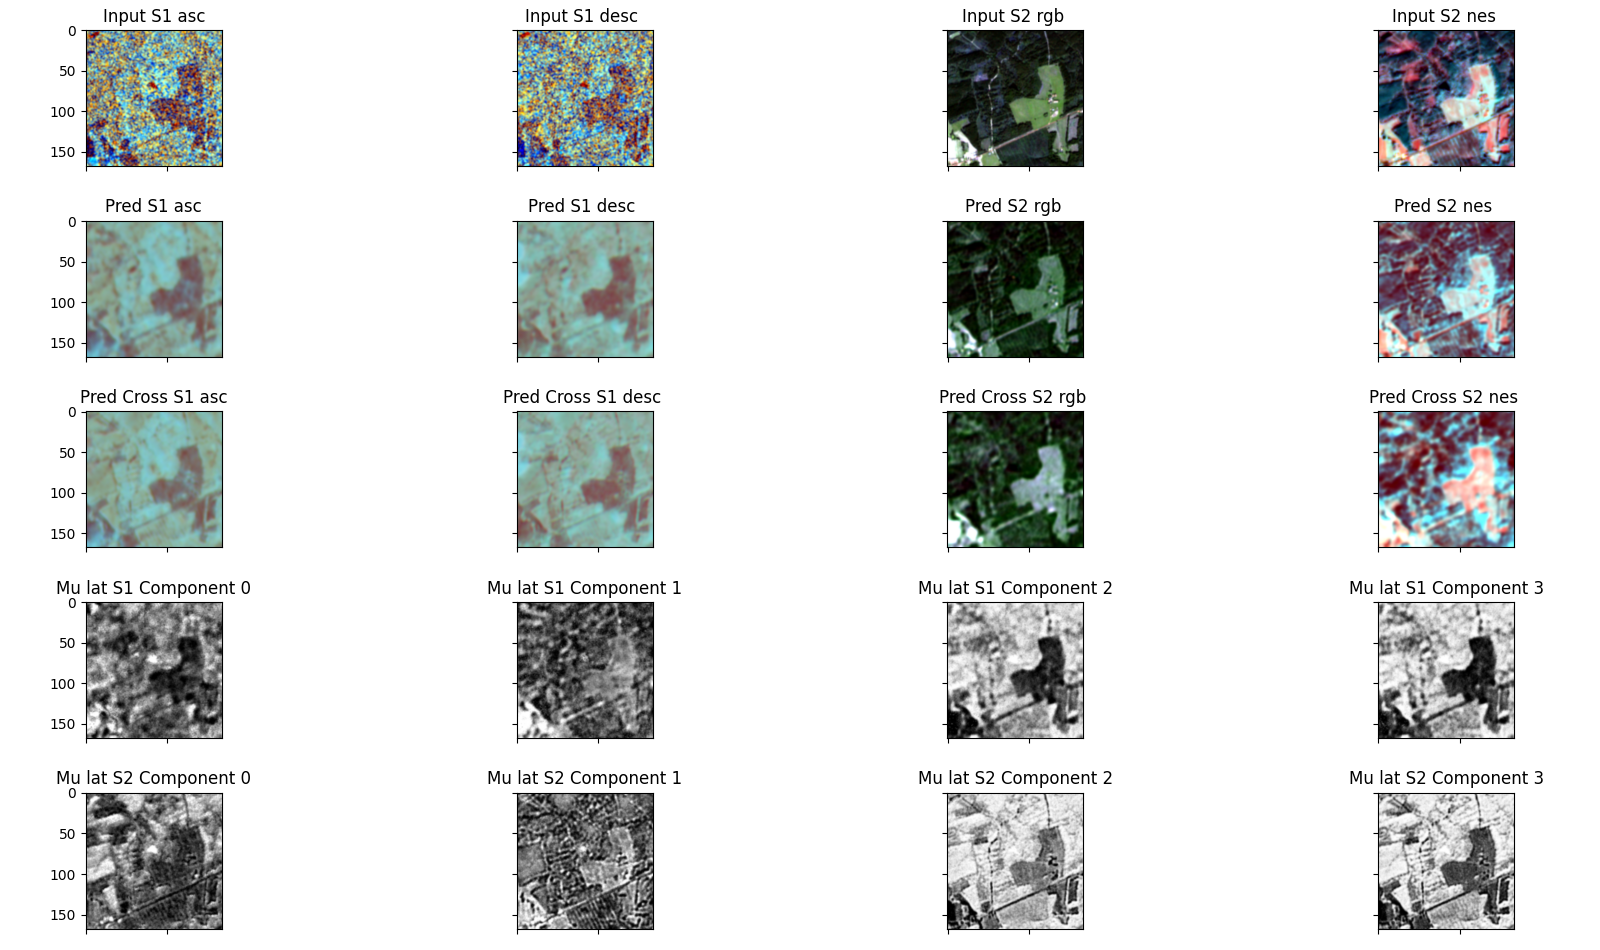
\includegraphics[width=\columnwidth]{img/wp1/mmdc5.png}
\caption{Illustration des données produites par le modèle MMDC. En colonnes, de gauche à droite, image Sentinel-1 ascendante, image Sentinel-1 descentante, image Sentinel-2 (RVB) et image Sentinel-2 (IR). En lignes, de haut en bas, données originales, réconstructions directes, reconstructions latentes, espace latent Sentinel-1 et espace latent Sentinel-2.}
\label{fig:mmdcresults}
\end{center}
\end{figure}

\paragraph{Architecture du modèle.}
Le modèle MMDC retenu est un auto-encodeur variationnel multi-modal, similaire à la méthode de cross-génération de \cite{shi-2019-variat-mixtur}. Un encodeur par modalité est utilisé afin d’engendrer un espace latent gaussien. Un décodeur par modalité est aussi utilisé por réconstruire les données d’entrée. Les décodeurs peuvent être des réseaux de neurones ou des modèles physiques sans entrainement. Dans ce dernier cas, l’espace latent représente les variables d’entrée des modèles physiques. Dans le cas où les décodeurs sont des réseaux de neurones, l’espace latent n’a pas d’interprétation. Une illustration de ce dernier cas est donnée sur la figure \ref{fig:mmdcresults}.

L’entraînement du modèle se fait par optimisation d’une fonction de coût composée de 5 termes :
\begin{itemize}
\item 2 termes correspondant aux erreurs de réconstruction directes (encodage S1 suivi de décodage S1, et de même pour S2) ;
\item 2 termes correspondant aux erreurs de réconstruction croisées (encodage S1 suivi de décodage S2, et son réciproque) ;
\item 1 terme de divergence entre les espaces latents générés par les 2 encodeurs pour une paire de données S1 et S2.
\end{itemize}

Les erreurs de réconstruction sont mesurées par une log-vraisemblance gaussienne et la divergence entre les espaces latents est mesurée avec la divergence de Kullback-Leibler entre les distributions (gaussiennes) inférées par les encodeurs. On se rapproche ainsi du ELBO classique dans les VAE adapté pour le cas multi-modal et où l’espace latent de chaque modalité agit en tant que prior de la modalité complémentaire.

Il est intéressant de noter la donnée S1 est composée des orbites ascendante et descendante de la même date (à 12h d’écart). Dans le cas où une seule orbite serait disponible (hors Europe, le plan d’acquisition de S1 ne garantit pas la présence des 2 images) la donnée est mise à zéro en utilisant la stratégie de \textit{modality dropout} \cite{neverova-2016-moddr}.

Les données satellite sont constituées des mesures (bandes spectrales optiques et polarisations SAR), mais aussi des informations de géométrie d’acquisition (angles capteur et solaires en optique et angle d’incidence locale en SAR). Ces données sont complétées par des informations de topographie (altitude, pente et aspect issus du modèle numérique de terrain SRTM) et des variables climatiques de la base de données Worldclim2 \cite{fick17_world}.

\paragraph{Préparation de jeux de données multimodaux de pré-entraînement.}

L’entraînement de modèles de fondation du type MMDC nécessite des gros volumes de données. Nous avons constitué un jeu de données dont le volume dépasse les 2TB. Il est composé de toutes les données disponibles sur l’année 2018 pour les capteurs Sentinel-1 et Sentinel-2 sur 50 tuiles de la grille MGRS sélectionnées de façon aléatoire sur l’ensemble des surfaces continentales de façon à couvrir des zones climatiques et des paysages différents. Elles sont illustrées sur la figure \ref{fig:mmdctiles}. Sur chacune de ces tuiles, 5 régions d’intérêt (ROI) de 1024 $\times$ 1024 pixels (à 10$\:$m. de résolution spatiale) sont découpées de façon aléatoire. Toute la profondeur temporelle est conservée. Chaque ROI est accompagnée des 103 variables climatiques Worldclim2 et du Modèle Numérique de Terrain (MNT) SRTM. Le code source utilisé pour la constitution du jeu de données est disponible \href{https://src.koda.cnrs.fr/mmdc/mmdc-datacollection}{en ligne}.


\begin{figure}[htbp]
\begin{center}
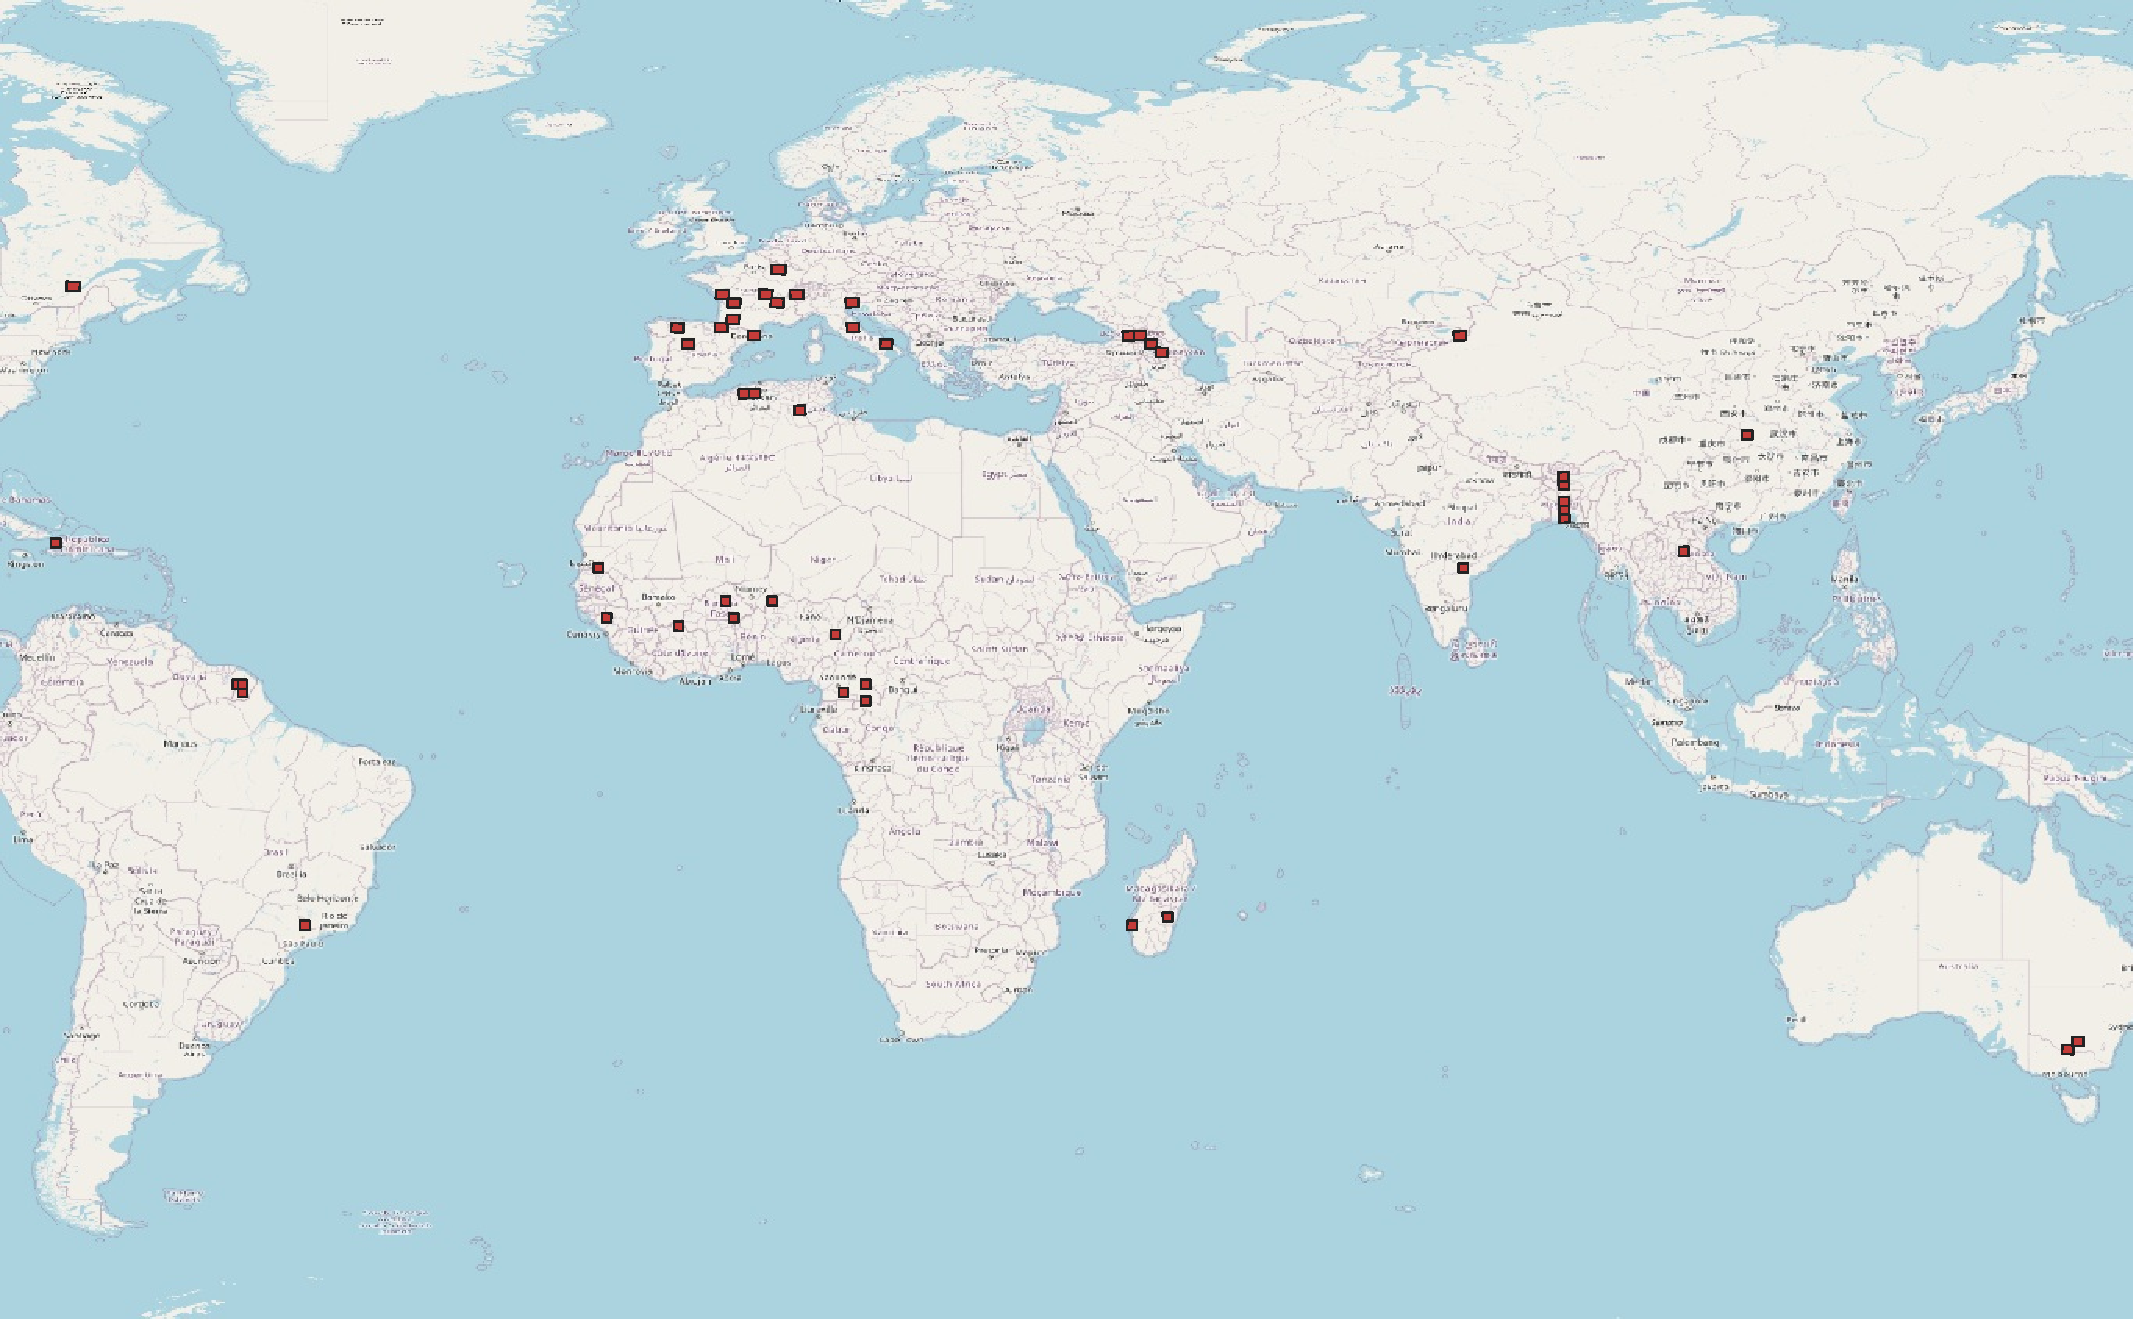
\includegraphics[width=\columnwidth]{img/wp1/tiles.pdf}
\caption{Localisation des 50 tuiles MGRS sélectionnées pour le jeu de données MMDC.}
\label{fig:mmdctiles}
\end{center}
\end{figure}

Au delà des travaux prévus dans MAESTRIA, ces données ont pu être valorisées dans \citep{dumeur-2023-self-satel}.

\paragraph{Code source.}
L’ensemble du code dévelopé dans le cadre du WP1 est disponible en ligne sur \href{https://src.koda.cnrs.fr/mmdc}{Koda CNRS} . Nous avons utilisé la bibliothèque \href{https://pytorch.org/}{Pytorch} pour la mise en œuvre des modèles de réseaux de neurones, l’orchestration des apprentissages a été faite avec la bibliothèque \href{https://lightning.ai/}{Pytorch Lightning} et toutes les expériences ont été configurées et paramétrées avec la bibliothèque \href{https://hydra.cc/}{Hydra}.

Le code a été décomposé en plusieurs dépôts, dont \href{https://src.koda.cnrs.fr/mmdc/mmdc-singledate}{le principal} contient les modèles de réseaux de neurones.

Nous avons aussi réalisé le portage en Pytorch du modèle de transfert radiatif PROSAIL \cite{jacquemoud-2009-prosp-sail-model} à partir de sa version Numpy \cite{domenzain19}. Ceci a été nécessaire pour pouvoir insérer le modèle physique dans les modèles d’apprentissage profond. En effet, pour réaliser l’apprentissage de bout en bout, il est nécessaire de rétro-propager les gradients des fonctions de coût à travers toutes les opérations du modèle (encodeurs et décodeurs). Dans le cas de l’apprentissage avec a priori physiques, le décodeur est remplacé par le modèle physique, qui doit être différentiable et capable de propager les gradients.

\paragraph{Intégration dans $\iota^2$.}
Afin de pouvoir déployer les modèles MMDC sur de grandes étendues, MAESTRIA a proposé de faire des évolutions à la chaîne $\iota^2$ développée initialement par le CESBIO. L’idée principale a était d’utiliser les encodeurs MMDC comme extracteurs de primitives qui pourraient être insérés dans le workflow $\iota^2$ (extraction de primitives, apprentissage, inférence). $\iota^2$ étant un projet existant avec des pratiques de développement ouvertes \href{https://framagit.org/iota2-project/iota2}{sur une forge publique}, les développements nécessaires à MAESTRIA ont été découpés en tickets spécifiques :
\begin{itemize}
\item création de data-loaders pour entraîner des modèles de réseaux de neurones dans $\iota^2$ (\href{https://framagit.org/iota2-project/iota2/-/issues/194}{ticket 194});
\item prise en compte de l’échantillonnage irrégulier dans les séries temporelles (\href{https://framagit.org/iota2-project/iota2/-/issues/318}{ticket 318});
\item prise en compte d’échantillons sous forme de patchs pour les CNN (\href{https://framagit.org/iota2-project/iota2/-/issues/334}{ticket 334});
\item calcul de statistiques et standardisation des données dans les data-loaders (\href{https://framagit.org/iota2-project/iota2/-/issues/418}{ticket 418});
\item profilage et optimisation des fonctionnalités d’apprentissage profond (\href{https://framagit.org/iota2-project/iota2/-/issues/579}{ticket 579}).
  
\end{itemize}


\subsubsection{Apprentissage grande échelle}
Les travaux du WP2 concernaient le développement d'une méthode d'apprentissage adapté au contexte MAESTRIA: multi-source, grande échelle spatiale et volume de données massif. En particulier, nous avions comme objectif de gérer des données d'apprentissage bruitées (avec des labels incorrects) et de pouvoir extraire des informations statistiques des classe (e.g., multi-modalité et variabilité spatiale).

Les travaux se sont orientés vers la définition d'un algorithmes semi-supervisé permettant d'exploiter le volume important de données satellites disponibles, avec ou sans label. Comme hypothèse de départ, nous avons supposé qu'un clustering non-supervisé des données dans le domaine spectral était disponible. C'est à dire que pour chaque pixel à traiter, la probabilité d'appartenance à \(K\) clusters \(S\) était disponible. Cette hypothèse correspond à un modèle de mélange classique dans la littérature:

\[p(\mathbf{x}) = \sum_{j=1}^Kp(X=\mathbf{x}|S=j)p(S=j).\]

Un fois les clusters supposés connus, le problème d'apprentissage revient à estimer la probabilité \(r_{ij}\) qu'un cluster \(j\) appartient à la classe \(i\), avec \(i\in\{1, \ldots,k\}\). L'idée sous jacente était d'exploiter la structure par clusters des données pour limiter l'effet d'échantillons mal labélisé dans la bases de données, en réalisant une classification des densités de probabilité (les clusters) plutôt que de leur réalisation (les pixels, dont les outliers).

En utilisant le modèle \emph{robust mixture discriminant analysis} (RMDA) de~\cite{bouveyron-2009-robus-super}, il est possible d'estimer \(r_{ij}\) en minimisant la log-vraisemblance du modèle RMDA:
\begin{eqnarray}
  \label{eq:ll}
  \begin{array}{rl}
    \displaystyle{\min_{\mathbf{R}}}
   &\displaystyle{\sum_{\ell=1}^n -\ln\big(\boldsymbol{\beta}_\ell^\top\mathbf{R}\boldsymbol{\psi}_\ell\big)},\\
   \text{Constraint to} & \mathbf{R}^\top\mathbf{1}_C = \mathbf{1}_K,\\
  & \mathbf{R} \succcurlyeq 0,
  \end{array}
\end{eqnarray}
où \(\boldsymbol{\psi}_\ell\) est le vecteur d'appartenance au \(K\) clusters du pixel \(\ell\), \(\boldsymbol{\beta}_\ell\) est le vecteur \emph{one-hot-encoded} d'appartenance à la classe du pixel \(\ell\) (\(\beta_{\ell i}=1\) si \(i=c_\ell\), sinon \(\beta_{\ell i}=0\)),  \(\mathbf{R}\in\mathbb{R}^{k\times K}\) la matrice des probabilités \(r_{ij}\), \(\succcurlyeq\) dénote la contrainte de non-négativité élément par élément de \(\mathbf{R}\) et \(\mathbf{1}_k\in\mathbb{R}^k\) un vecteur contenant la valeur 1.

Nous avons montré dans un premier temps que ce problème était un problème d'optimisation convexe, en calculant la matrice Hessienne de~(\ref{eq:ll}) et en observant qu'elle était définie semi-positive~\citep[Section~3.1]{GIRYFOUQUET2021320}.

A partir de là, nous avons transformer ce problème d'optimisation en un problème d'optimisation par consensus en découplant le problème en sous-problèmes plus simples à résoudre et en définissant une variable globale sur laquelle la contrainte du simplexe était imposée:

\begin{eqnarray}
  \label{eq:consensus}
   \begin{array}{rl}
     \displaystyle{\min_{\mathbf{R}_\ell,\mathbf{Z}}} & \displaystyle{\sum_{\ell = 1}^{n}f_\ell(\mathbf{R}_\ell)} + g(\mathbf{Z}),\\
     \text{Constraint to} & \mathbf{R}_\ell - \mathbf{Z} = \mathbf{0}\ \forall \ell\in\{1,\ldots,\ n\},
   \end{array}
\end{eqnarray}
où \(f_\ell(\mathbf{R}_\ell)  = -\ln(\boldsymbol{\beta}_\ell^\top\mathbf{R}_\ell\boldsymbol{\psi}_\ell)_{+}\) pour \(\ell\in \{1,\ldots,n\}\), \((\cdot)_{+}=\max(0, \cdot)\) et \(g(\mathbf{Z})\) est définie comme la fonction indicatrice sur le simplexe \(\mathcal{S}\):
\begin{eqnarray}
  g(\mathbf{Z})  =  \left\{
                      \begin{array}{rl}
                        0 & \text{ si } \mathbf{Z}\in\mathcal{S} = \{\mathbf{Z}|\mathbf{Z}\succcurlyeq 0, \mathbf{Z}^\top\mathbf{1}_C = \mathbf{1}_{K}\}, \\
                        +\infty & \text{ sinon.} 
                      \end{array}
                                  \right.                                  \label{eq:simplex}
\end{eqnarray}
Cette formulation permet d'appliquer l'algorithme ADMM~\cite[Chapter~7]{boyd-2010-distr-optim}. Dans cadre, le Lagrangien augmenté s'écrit:
\begin{multline}
  \mathcal{L}_{\rho}(\mathbf{R}_1,\ldots,\mathbf{R}_n,\ \mathbf{Z},\mathbf{Y}_1,\ldots,\mathbf{Y}_n) = \\ \sum_{\ell=1}^{n} \Bigg(f_{\ell}(\mathbf{R}_\ell) + \langle\mathbf{Y}_\ell, \mathbf{R}_\ell - \mathbf{Z}\rangle_F + \frac{\rho}{2}\|\mathbf{R}_\ell - \mathbf{Z}\|^2_F\Bigg) + g(\mathbf{Z}),
  \label{eq:consensus:lagrangian}  
\end{multline}
où \(\mathbf{Y}_\ell\) sont les multiplicateurs de Lagrange, \(\langle\cdot,\cdot\rangle_F\) est le produit scalaire de Frobenius entre deux matrices réelles, \(\|\cdot\|_F\) sa norme associée et \(\rho\) un paramètre de pénalité. L'algorithme itératif résultant est le suivant:
\begin{align}
  \mathbf{R}_{\ell}^{(t+1)} = {} &  \begin{aligned}[t]
    \arg\min_{\mathbf{R}_\ell}\Bigg\{ & f_{\ell}(\mathbf{R}_\ell) + \langle\mathbf{Y}_\ell^{(t)}, \mathbf{R}_\ell - \mathbf{Z}^{(t)}\rangle_F  + \frac{\rho^{(t)}}{2}\|\mathbf{R}_\ell - \mathbf{Z}^{(t)}\|^2_F\Bigg\},
  \end{aligned}\label{eq:consensus:Rl}\\
  \mathbf{Z}^{(t+1)}  = { }&   \begin{aligned}[t]
    \arg\min_{\mathbf{Z}}\Bigg\{ & g(\mathbf{Z}) + \sum_{\ell=1}^{n} \bigg(\langle\mathbf{Y}_\ell^{(t)}, \mathbf{R}_\ell - \mathbf{Z}\rangle_F   + \frac{\rho^{(t)}}{2}\|\mathbf{R}_\ell^{(t+1)} - \mathbf{Z}\|^2_F\bigg)\Bigg\},
  \end{aligned}\label{eq:consensus:Z}\\
  \mathbf{Y}^{(t+1)}_\ell = {} &\mathbf{Y}^{(t)}_\ell + \rho^{(t)}\big(\mathbf{R}_\ell^{(t+1)}-\mathbf{Z}^{(t+1)}\big), \label{eq:consensus:Y}
\end{align}
où \((t)\) indiques l'itération courante. Cet formulation est efficiente car chaque étape de mise à jours peut se paralléliser massivement, et être obtenue analytiquement. Les étapes de mises à jours sont décrites dans~\cite{GIRYFOUQUET2021320}.

Cette algorithme a été implémenté en Python avec le compilateur JIT Numba (\mathieu{Rajouter lien vers gitlab quand réparé}). Par rapport au solveur de \cite{bouveyron-2009-robus-super}, la solution proposée est jusqu'à 400 fois plus rapide. Sur un ordinateur portable standard, un problème avec 10 classes, 100 clusters et 10 millions de pixels est résolu en 20 minutes environ.

Les résultats sur des jeux de données simulés montrent une grande robustesse vis à vis du bruit dans les labels, avec un maintient des performances jusqu'à 50\% des labels corrompus. Cependant, sur des données de télédétection réelles, la tache de clustering limite les performances globales: si les clusters sont mal définies (par exemple, plusieurs classes regroupé dans un même cluster) les performances en terms de taux de bonnes classification seront faibles.

Pour pallier à cette faiblesse, nous avons avons utilisé la dérivabilité de log-vraisemblance pour inclure cette formulation dans un auto-encoder (AE) et définir une étape de clustering dans l'espace latent. Le problème d'apprentissage consiste alors à optimiser une partie du modèle avec une fonction de coût classique des AE (reconstruction) et une fonction de coût de clustering, puis d'optimiser la log-vraisemble du modèle robuste avec la formulation discuté plus haut. Nous avons obtenue une amélioration des résultats de classification, mais cependant, pas assez pour arriver à l'état de l'art.

\subsubsection{Dérivation de produits adaptés à des utilisateurs finaux}
Cette tâche devait bénéficier des avancées méthodologiques amont des deux tâches précédemment décrites dans deux directions (D) particulières:
\begin{itemize}
    \item[\textbf{D1:}] exploiter la flexibilité offerte et les performances de classification améliorée pour dériver un plus grand nombre d'occupation des sols à des échelles spatiales et sémantiques plus importantes. Cela devait se décliner en deux sous-objectifs:
    \begin{itemize}
        \item[\textbf{D1.1:}]  développer des méthodes afin de passer d'un ensemble restreint de cartes OCS à une gamme plus large, de manière automatique, sans avoir de nouveau recours à des processus de classification (apprentissage et extraction d'informations) coûteux;
        \item[\textbf{D1.2:}] organisation de trois colloques avec des utilisateurs finaux pour d'abord préciser les spécifications attendues dans différents domaines et enfin valider les OCS générées. 
    \end{itemize}
    \item[\textbf{D2:}] implémenter toutes les méthodes dans un cadre commun ouvert, proposer des produits adaptés aux différents utilisateurs finaux, et ouvrir ces produits également de manière libre.
\end{itemize}

La tâche D1.1 a pu être menée à bien sans tenir compte de la réduction des ambitions des tâches de fusion et d'apprentissage large-échelle bruité. Elle est décrite ci-dessous, sous le concept de "\textit{traduction de cartes d'OCS}". Toutefois, la tâche D1.2 s'est limitée à l'organisation d'un workshop initial, 1 mois avant le déclenchement de l'épidémie de COVID-19. L'absence de produits, de contributions méthodologiques fortes et de spécifications précises édictées ont obéré la tenue de workshops intermédiaires et la nécessité d'impliquer des utilisateurs finaux.

\subsubsection*{Apprentissage de traduction de cartes d'OCS}
De multiples cartes d'OCS sont désormais produites automatiquement par analyse d'images géospatiales. souffrent toutefois de deux inconvénients limitant leur utilisation. D'une part, la résolution spatiale est fixe. Or une carte d'une résolution de 10 mètres ne conviendra pas à l'analyse de phénomènes à grande échelle, ni à l'étude d'objets de moins de 10 mètres. D'autre part, la nomenclature est choisie pour répondre à un besoin spécifique qui ne correspond pas nécessairement aux besoins d'un autre utilisateur. Ainsi, une carte peut regrouper sous le terme "\textit{bâti}" un ensemble d'éléments tels que des "rout\textit{}es" et des "\textit{habitations}", qui dans d'autres nomenclatures seront classés séparément.
       
Les approches actuelles de traduction de nomenclatures sont principalement fondées sur des méthodes de traduction sémantique (LCCS\ldots) appliquées au niveau de la nomenclature en comparant les définitions de classes (la classe "\textit{blé}" sera traduite en "\textit{herbacée}"). Le lecteur pourra par exemple se référer à ~\cite{DiGregorio1998}, \cite{Jepsen2013}, \cite{Adamo2014}, ou \cite{Li2020}. Elles négligent le fait que deux objets de la même classe peuvent être traduits différemment en fonction, par exemple, de leur contexte spatial ou de leur évolution temporelle. En outre, la traduction de la résolution spatiale est généralement traitée distinctement de la traduction de nomenclature alors que ces deux notions sont intimement liées (un arbre seul ne peut pas être traduit en "\textit{forêt}").
       
Nous avons abordé ce problème en proposant des méthodes de traduction (source $\rightarrow$ cible), contextuelle, augmentant les possibilités de réutilisation et de génération de nouvelles occupations des sols et traitant conjointement les transferts de résolution et de sémantique. Nous avons identifié quatre principaux types de contexte: (i) le contexte spatial (incluant les caractéristiques des objets et les relations entre ces derniers), (ii) le contexte géographique, (iii) le contexte temporel (cas des classes définies avec une notion de durée), (iv) la structure du bruit des classes, spécifique à chaque OCS (ou contexte cartographique).\\
     \begin{figure}[htbp]
        \centering%
        \includegraphics[width=0.96\textwidth]{img/wp3/main_idea-2.pdf}
       \caption{Architecture pour une traduction multi-OCS. Notre réseau (en bleu) est entraîné pour traduire et auto-reconstruire les cartes en entrée (ici avec deux cartes A et B). Les flèches rouge et orange représentent les chemins possibles pour A et B, e.g., A peut soir être traduite vers B, soit être reconstruite. \`A l'inférence, une seule carte source est nécessaire.\label{fig:mlctnet}.}
        \end{figure}
Dans un premier temps, nous avons proposé différentes stratégies 1-1, principalement fondées sur des réseaux de neurones à convolution (U-Net asymmétrique) apprenant à traduire une carte source en une carte cible en fonction du contexte. Nous avons montré l'importance cruciale du contexte spatial et géographique, avec l'intégration d'un module d'encodage des coordonnées géographiques des images générées à partir des OCS, sur de multiples exemples de traductions (une forêt en montagne est probablement constituée de conifères). La comparaison par rapport à six méthodes standard, adaptées de la littérature, a également validé la pertinence de notre méthode, autant quantitativement que qualitativement \cite{Luc_RS}, tout comme la pertinence d'apprendre les attributs spatiaux discriminants plutôt que de les prédéfinir et les calculer en amont. L'application au cas de la traduction de la carte européenne Corine Land Cover à partir de la classification pixellaire annuelle OSO a montré la possibilité de fournir une OCS Corine Land Cover (CLC) à l'échelle de la France en une douzaine d'heures (alors qu'aujourd'hui CLC est fournie tous les 6 ans en Europe). \\

Dans un deuxième temps, partant du constat que les modèles de traduction multi-langues donnent de meilleurs résultats que ceux entraînés à traduire d'une seule langue source vers une seule langue cible \cite{Pires2019}, nous proposons un modèle de traduction multi-cartes ($n$-$n$ nommé  \textit{Multiple Land-Cover Translation Network},MLCT-Net), permettant d'obtenir plusieurs nomenclatures cibles à partir d'une carte source, toujours en suivant le principe d'encodeur-décodeur. Il n'y a pas de restriction sur le nombre de cartes construisant l'espace de représentation communs (nous sommes montés jusqu'à 10). On s'est fondé sur deux principes simples: l'encodeur doit avoir un champ réceptif suffisamment large pour encoder les objets géographiques avec leur contexte et le décodeur doit être suffisamment simple pour que l'espace commun de représentation appris soit aussi identique que possible aux OCS en entrée (Figure~\ref{fig:mlctnet}.
Nous avons montré que ce modèle permettait d'obtenir des résultats plus robustes que les modèles entraînés sur une seule traduction, en particulier sur des cartes avec peu d'échantillons d'entraînement \cite{Luc_IGARSS22} \cite{luc_ijgis}. D'un point de vue opérationnel, en particulier, ce modèle permet d'obtenir en quelques heures, à l'échelle de la France, des OCS produites uniquement sur des territoires restreints (dans notre cas, département ou région française).\\
  \begin{figure}[htbp]
        \centering
        \includegraphics[width=\textwidth]{img/wp3/comparaison.png}
        \caption{Comparaison visuelle entre la méthode MLCT-Net (\textit{Multi-LC}), la méthode 1-1 (\textit{Mono-LC}) et deux méthodes de l'état de l'art (\textit{Statistic} et \textit{Semantic}) sur les différentes OCS de notre jeu de données (nommées ici CGLS, CLC, OSO, MOS, G1 et G2).\label{fig:comparison}}
        \end{figure}
Troisièmement, nous avons expérimenté différentes configurations de fusion multimodale au sein de MLCT-Net (amont, aval, intermédiaire) intégrant des images satellites (optiques et radar) et des données d'élévation du terrain avec des cartes d'occupation du sol, dans l'objectif premier d'affiner spatialement les cartes produites, avec l'insertion d'un mécanisme d'attention par canal et donc la pondération automatique des informations annexes fournies. Cela a résulté en 39 modèles testés, avec une préférence pour une fusion tardive et une légère préférence pour l'imagerie Sentinel-2 mono-date. On a conclu que la fusion entre des images et notre espace de représentation n'est pertinent que dans le cas où la source a une résolution spatiale équivalente ou plus fine que l'OCS cible.\\

Enfin, nous avons défini la notion et avons proposé une méthode pour construire un \textit{espace de représentation sémantique commun} à toutes les occupations du sol. Nous ne représentons alors plus la traduction comme le passage d'un espace de représentation discret à $n$ classes (une nomenclature) vers un autre espace, mais comme un simple changement d'interprétation d'un espace de représentation sémantique continu commun à toutes les nomenclatures. Nous nous sommes fondés sur l'encodage de la définition des classes d'OCS (Bag-of-Words, Word2Vec et Transformers, cf. \cite{Comber2015}, \cite{Pradhan2020}, \cite{Wang2020}), sa réduction et la définition de métriques pour calculer la proximité entre classes Nous avons alors proposé une première application de la notion d'espace de représentation sémantique à la traduction, en nous concentrant sur la traduction de cartes sources non vues pendant l’entraînement du modèle de traduction. Cela offre désormais la possibilité de traduire toute nouvelle carte fournie par un utilisateur final, avec une nomenclature non connue.\\

Dans les approches présentées ci-dessus, les qualités obtenues sont très généralement au niveau, ou légèrement supérieures, aux qualités fournies ou estimées par nous-mêmes pour les occupations du sol que nous avons cherché à traduite (aux alentours de 80-85\%). \'Evidemment, les scores fluctuent selon les classes, selon leur complexité inhérente (liée à leur définition) ou leur forte ou rare présence dans les cartes.\\
Ce travail a nécessité pour cela l'établissement de vérités terrain indépendantes des OCS testées, afin d'évaluer une qualité au-delà de la capacité des méthodes à répliquer les erreurs inhérentes aux OCS. Selon un processus identique, la première annotation par interprétation visuelle a conduit à 5000 points (pour la traduction 1-1) et la deuxième à 2300 points (pour MLCT-Net).

Les codes et jeux de données (France entière, six cartes d'occupation du sol, images satellite, vérité terrain, nommés MLULC) produits au cours de cette thèse ont été rendus accessibles pour la reproductibilité et des comparaisons futures (cf. Section~\ref{subsec:valo}).


\subsection{Exploitation des résultats}
Les travaux menés sur la fusion de données (WP1) sont couplés avec les avancées méthodologiques du projet ANR en cours \href{https://anr.hal.science/search/index/?q=*&anrProjectReference_s=ANR-20-CE23-0003}{DeepChange} (ANR-20-CE23-0003). Ce dernier a débuté 2 ans plus tard et bénéficie donc des réflexions et travaux préliminaires menés dans le cadre de MAESTRIA, tout comme la chaîne $\iota^2$ a bénéficié d'un certain nombre de fonctionnalités nécessaires au déploiement des modèles MMDC. En conséquence, avec une forge ouverte, ces résultats sont à la disposition des communautés scientifiques ainsi que des industriels travaillant également sur l'exploitation des images d'observation de la Terre.\\
Les mêmes conclusions s'appliquent aux travaux des WP2 et WP3. Les développements du WP3 pourraient être repris par le Service d'Innovation de l'Institut National de l'Information Géographique et Forestière (IGN), une des tutelles du LASTIG, afin de générer automatiquement des OCS à différentes échelles spatiales à partir d'une OCS pixellaire à 0,2$\:$m de résolution obtenue automatiquement par apprentissage profond \cite{garioud2023flair}, \cite{garioud2023flair2}.


\subsection{Discussion} 
Au vu des résultats et de leur exploitation détaillés ci-dessus, on peut conclure que seulement une partie des objectifs du projet ont été atteints. La crise sanitaire et la non finalisation de 2 thèses sur les trois de MAESTRIA ont fortement négativement impactés le projet et les valorisations escomptées: d'une part, l'intégration des résultats dans $iota^2$ par un ingénieur dédié et d'autre part la production d'OCS à partir des briques des trois workpackages pour un dialogue avec des utilisateurs finaux. Sans briques méthodologiques, nous avons dû ainsi abandonner la tenue de colloques avec des utilisateurs finaux et prescripteurs pour leur communiquer les résultats du projet et récolter les spécifications des produits attendus. 

Ceci étant dit, d'un point de vue méthodologique, avec un recul de 6 ans par rapport à la construction initiale du projet, il s'avère que les problématiques identifiées étaient cohérentes et restent d'actualité. Peu de réorientations auraient été objectivement nécessaires si les tâches avaient pu être menées à bien. Les deux incertitudes initiales majeures étaient (i) la capacité à articuler les résultats des trois tâches et (ii) l'intégration de techniques d'apprentissage profond, peu matures en 2018 pour traiter des séries temporelles d'observation de la Terre. Les résultats actuels ont montré notre capacité à les intégrer et à développer des solutions innovantes.

L’autre objectif insuffisamment atteint concerne l’application concrète des résultats du projet à divers cas d’usage identifiés ou à identifier avec des utilisateurs finaux. Toutefois, nous avons pu constater ces dernières années une montée en maturité de briques méthodologiques fondées sur l'apprentissage profond pour la génération de cartes d'OCS à des échelles de plus en plus large et le déploiement de solutions opérationnelles chez de nombreux opérateurs publics et privés. La dynamique actuelle est donc très positive pour continuer nos travaux, qui restent d'actualité.

\subsection{Conclusions}
Le projet MAESTRIA a permis aux laboratoires LASTIG et CESBIO de progresser sur différents aspects de l'analyse automatique d'images satellites multimodales pour la génération de cartes d'occupation du sol. Le co-encadrement des travaux de recherche a permis des échanges fructueux et aux partenaires de profiter de leurs complémentarités. L'ambition initiale du projet était la bonne, ni trop haute ni trop basse, et la plupart des sujets qui auraient dû être traités sont aujourd'hui encore très prégnants et assez ignorés dans la littérature scientifique.

